\documentclass[20pt]{article}
\usepackage[utf8]{inputenc}
\usepackage[warn]{mathtext}
\usepackage[russian]{babel}

\usepackage{natbib}

\usepackage{caption}
\usepackage{graphicx}
\graphicspath{}
\DeclareGraphicsExtensions{.pdf,.png,.jpg}
\DeclareSymbolFont{T2Aletters}{T2A}{cmr}{m}{it}
\usepackage{subcaption}

\begin{document}
\begin{minipage}{0.8\textwidth}
\begin{center}
    \large{Санкт-Петербургский национальный исследовательский университет информационных технологий, механики и оптики
\\УЧЕБНЫЙ ЦЕНТР ОБЩЕЙ ФИЗИКИ ФТФ}
\medbreak
\end{center}
\end{minipage}
\hfill
\begin{minipage}{0.3\textwidth}

\includegraphics[scale=0.4]{itmo.jpg}
\end{minipage}

\noindent\rule{\textwidth}{1pt}
\medbreak
\begin{minipage}{0.5\textwidth}
Группа $\textit{P3112}$						
\\Студент $\textit{Сенина Мария Михайловна}$			
\\Преподаватель $\textit{Сорокина Е К}$
\end{minipage}
\hfill
\begin{minipage}{0.4\textwidth}
К работе допущен
\\Работа выполнена
\end{minipage}

\bigbreak

\begin{center}
        \Large{\textbf{Рабочий протокол и отчёт по лабораторной работе №3}}
   \LARGE{\textbf{\\ Изучение центрального соударения двух тел. Проверка второго закона Ньютона}}
\end{center}

\section{Цель работы}
Изучение центрального соударения двух тел. Проверка второго
закона Ньютона.

\section{Задачи, решаемые при выполнении работы}
\begin{enumerate}
    \item Исследование упругого и неупругого центрального соударения тел на примере тележек,движущихся с малым трением.
    \item Исследование зависимости ускорения тележки от приложенной силы и массы тележки.
\end{enumerate}

\section{Объект исследования}
Соударение двух тележек на рельсе

\section{Метод экспериментального исследования}
\subsection*{Часть 1}
Будем сталкивать две тележки, движущиеся по рельсу с малым трением. В начале одна из которых покоится. При абсолютно упругом столкновении сохраняется и энергия и импульс системы:
% m_1\overrightarrow{v_{10}} = m_1\overrightarrow{v_1} + m_2\overrightarrow{v_2} \\
% \frac{m_1 v_{10}^2}{2} = \frac{m_2 v_{1}^2}{2} + \frac{m_2 v_{2}^2}{2} 
\begin{equation*}
        \left\{ 
        \begin{array}{l}
            m_1\overrightarrow{v_{10}} = m_1\overrightarrow{v_1} + m_2\overrightarrow{v_2}\\
            \frac{m_1 v_{10}^2}{2} = \frac{m_2 v_{1}^2}{2} + \frac{m_2 v_{2}^2}{2}\\
        \end{array}
        \right. 
\end{equation*}
Так как соударение происходит на прямой можно ввести ось ОХ, сонаправленную со скоростью движения первой тележки, и уравнения вдоль этой оси останутся прежними: 
\begin{equation*}
        \left\{ 
        \begin{array}{l}
            m_1 v_{10} = m_1 v_{1x} + m_2 v_{2x}\\
            \frac{m_1 v_{10}^2}{2} = \frac{m_2 v_{1x}^2}{2} + \frac{m_2 v_{2x}^2}{2}\\
        \end{array}
        \right. 
\end{equation*}
Отсюда можно вывести, что скорости тележек после удара будут следующие: 
\begin{equation*}
        \left\{ 
        \begin{array}{l}
            v_1 = \frac{(m_1-m_2)v_{10}}{m_1 + m_2}\\
            v_2 = \frac{2 m_1 m_{10}}{m_1 + m_2}
        \end{array}
        \right. 
\end{equation*}.

\\ При этом, если мы рассматривем абсолютно не упругий удар, после которого обе тележки движутся вместе, как единое тело - законы сохранения импульса и энергии принимают следующий вид:  
\begin{equation*}
        \left\{ 
        \begin{array}{l}
            m_1\overrightarrow{v_{10}} = (m_1 + m_2)\overrightarrow{v}\\
            \frac{m_1 v_{10}^2}{2} = \frac{(m_1 + m_2)\overrightarrow{v}}{2} + W_{пот}\\
        \end{array}
        \right. 
\end{equation*}
где $W_{пот}$ - потеря мехарнической энергии в результате столкновения, а $\overrightarrow{v}$ - скорость новообрахованного тела, которая ровна $v = \frac{m_1 V_{10}}{m_1 +m_2}$. А знаичит $W_{пот} = \frac{m_1 m_2 v_{10}^2}{2(m_1 + m_2)}$. А $\delta_{W_{пот}} = \frac{W_{пот}}{\frac{m_1 v_{10}^2}{2}} = \frac{m_2}{m_1 + m_2}$
\subsection*{Часть 2}

\\Соберём установку, нарированную на рисунке $\ref{1}$ и распишем силы, действующие на тележку и соединённый с ней грузик. По второму закону Ньютона для тележки и грузика получаются следующие уравнения:

\begin{equation*}
        \left\{ 
        \begin{array}{l}
            \overrightarrow{a_1} = M\overrightarrow{g} + \overrightarrow{N} + \usepackage{T_1} + \overrightarrow{F_{тр}}\\
            m \overrightarrow{a_2} = m\overrightarrow{g} + \overrightarrow{T_2}\\
        \end{array}
        \right. 
\end{equation*}
Здесь $\overrightarrow{a_1}, \overrightarrow{a_2}$ - ускорения тележки и гирьки, $\overrightarrow{N}$ - сила реакции опоры, $\overrightarrow{F_{тр}}$ - сила трения и $\overrightarrow{T_1}, \overrightarrow{T_2}$ - силы натяжения нити, которые равны друг другу, потому что мы считаем нить нерастяжимой, а блок принебрежимо лёгким. По этой же причине модули ускорений тоже ровны. 

\begin{figure}[h]
\center{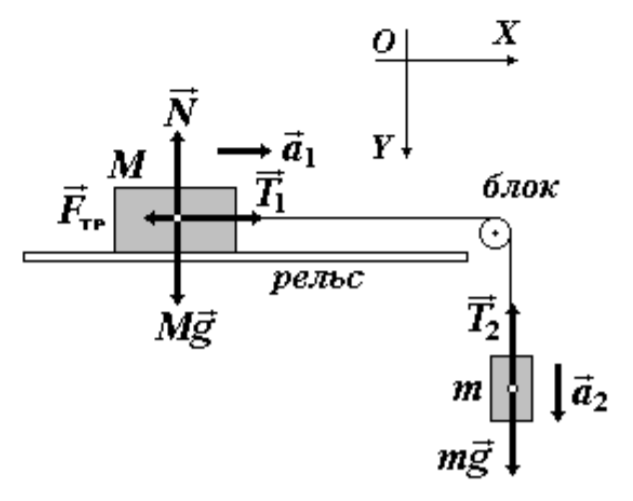
\includegraphics[scale=0.4]{схема.png}}
\caption{Схема установки}
\label{1}
\end{figure}

\\ Таким образом уравнения упрощаются: 
\begin{equation*}
        \left\{ 
        \begin{array}{l}
            OY: N = Mg\\
            OX: Ma = T - F_{тр}\\
        \end{array}
        \right. 
\end{equation*}

 \\ Значит, сила трения зависит от ускорения, как $T = Ma + F_{тр}$, значит, если сила трения не изменяется в ходе эксперимента - зависимость силы натяжения от ускорения - линейна, а угловой коэффицент этой зависимости равен $M$, а значение силы натяжения при нулевом ускорении ровна силе трения.
\section{Рабочие формулы и исходные данные}
\begin{enumerate}
    \item Импульс тела $\overrightarrow{p} = m\overrightarrow{v}$
    \item Закон сохраниния энергии для абсолютно упругого удара, такого что одно из тел в начале покоилось  $\frac{m_1 v_{10}^2}{2} = \frac{m_2 v_{1}^2}{2} + \frac{m_2 v_{2}^2}{2}$
    \item Закон сохранения энергии для абсолютно неупругого удара, такого, что одно из тел до удара покоилось $\frac{m_1 v_{10}^2}{2} = \frac{(m_1 + m_2)\overrightarrow{v}}{2} + W_{пот}$
    \item $\textbf{Формулы для абсолютно упрогого столкновения}$
    \begin{enumerate}
         \item Относительное изменение импульса $\delta_p = \frac{\Delta p_x}{p_{10x}} = \frac{(p_{1x} + p_{2x})}{p_{10x}} - 1$
        \item Относительное изменение кинетической энергии $\delta_W = \frac{\Delta W_k}{W_{k0}} = \frac{m_1 v_{1x}^2 + m_2 v_{2x}^2}{m_1 v_{10x}^2} - 1$
    \end{enumerate}
    \item $\textbf{Формулы для абсолютно не упругого столкновения}$
    \begin{enumerate}
        \item Импульс системы до соударения $p_{10} = m_1 v_{10}$\\
        \item Импульс системы после соударения $p =(m_1 + m_2) v$\\
        \item Относительное именение импульса $\delta_p = \frac{\Delta p}{p_{10}} =  \frac{p_1}{p_{10}} - 1$\\
        \item Экспериментальное значение относительного изменения механической энергии $\delta^{(э)}_W = \frac{\Delta W_к}{W_{к0}} = \frac{(m_1 + m_2) v_2^2}{m_1 v_{10}^2} - 1$\\
        \item Теретическое значение относительного изменения механической энергии $\delta^{(т)}_W = -\frac{W_{пот}}{\frac{m_1 v^2_{10}}{2}} = -\frac{m_2}{m_1 + m_2}$
    \end{enumerate}
    \item Среднее значение $\bar{x} = \frac{\sum\limits_{i=1}^N x_i}{N}$
    \item Погрешность измерений через коэффицент Стьюденса $\Delta x = t_{a_{дов, N}}\sqrt{\frac{\sum\limits_{i=1}^N (x - \bar{x})^2}{N (N-1)}}$, где $t_{a_{дов, N}}$ - коэффицент Стьюдентса для доверительной вероятности $a_{дов}$ и количества измерений $N$.
    \item Ускорение через скорость и координату $a = \frac{v^2_2 -v^2_1}{2(x_2 - x_1)}$
\end{enumerate}

\section{Измерительные приборы}
%ДОБАВИТЬ ИСПОЛЬЗУЕМЫЙ ДИАПАЗАОН
\begin{tabular}{p{0.5cm} | p{5cm} | p{3cm} | p{2cm} }\hline
# & Наименование & Используемый диапазон & Погрешность прибора \\ \hline
1 & Рельс с свнтиметровой шкалой на лицевой стороне  & ЧТО-ТО  & 5 мм \\  \hline
2 &	Цифровой измерительный прибор ПКЦ-3 & ЧТО-ТО & 	0,1 с \\   \hline
3 & Лабораторные электронные весы & ЧТО-ТО & 0,01 г \\ \hline
\end{tabular}

\section{Результаты прямых измерений и их \mbox{обработки}}
См. приложение 1.
\section{Расчёт результатов косвенных измерений}
См. таблицы в приложении 2.
\subsection*{Часть 1}
Я расчитала занчения импульсов тележек до и после соударения по формуле $\overrightarrow{p} = m\overrightarrow{v}$ в экспериментах с абсолютно упрогим столкновениям без утяжеления тележке (Таблица 1.1). А зная их вычслила относительное изменение импульса $\delta_p = \frac{\Delta p_x}{p_{10x}} = \frac{(p_{1x} + p_{2x})}{p_{10x}} - 1$ и его среднее значение $\bar{\delta_p} = \frac{\sum\limits_{i=1}^5 \delta_{p_i}}{5}$. И относительное изменение кинетической энергии $\delta_W = \frac{\Delta W_k}{W_{k0}} = \frac{m_1 v_{1x}^2 + m_2 v_{2x}^2}{m_1 v_{10x}^2} - 1$ и его среднее значение $\bar{\delta_W} = \frac{\sum\limits_{i=1}^5 \delta_{W_i}}{5}$.

\\ А дальше нашла погрешности $\Delta \bar{\delta_p}$ и $\Delta \bar{\delta_W}$ по формуле $\Delta \bar{\delta} = t_{a_{дов, 5}}\sqrt{\frac{\sum\limits_{i=1}^5 (\delta - \bar{\delta})^2}{5 (5-1)}}$, где $t_{a_{дов, 5}}$ - коэффицент Стьюдентса для доверительной вероятности $a_{дов}$ и количества измерений $N$.

\\ Аналогичным образом, я рассчистала погрешности и значения для экспериментов с абсолютноупругим столкновением, но с утяжелением тележек (Таблица 1.2):\\
$\bar{\delta_p} = , \Delta \bar{\delta_p} = $\\
$\bar{\delta_W} = , \Delta \bar{\delta_W} = $\\

\\ Далее для результатов экспериментов с абсолютно неупругим столкновнением без утяжеления тележек (таблица 2.1) по формулам ниже я вычислила значения для таблицы 5.1: \\
$p_{10} = m_1 v_{10}$ - импульс системы до соударения,\\
$p =(m_1 + m_2) v$ - импульс системы после соударения,\\
$\delta_p = \frac{\Delta p}{p_{10}} =  \frac{p_1}{p_{10}} - 1$ - относительное именение импульса,\\
$\delta^{(э)}_W = \frac{\Delta W_к}{W_{к0}} = \frac{(m_1 + m_2) v_2^2}{m_1 v_{10}^2} - 1$ - экспериментальное значение относительного изменения механической энергии, \\
$\delta^{(т)}_W = -\frac{W_{пот}}{\frac{m_1 v^2_{10}}{2}} = -\frac{m_2}{m_1 + m_2}$ - теретическое значение относительного изменения механической энергии

\\ А дальше через через формулы среднего и формулу погрешности через коэффцент Стьюденса вычислила:\\
$\bar{\delta_p} = , \Delta \bar{\delta_p} $\\
$\bar{\delta^{(э)}_W} = , \Delta \bar{\delta^{(э)}_W}$

\\Аналогичным образом я посчитала всё для эксперимента с абсолютно неупругим столкновением и утяжелением тележки (таблица 2.2):

$\bar{\delta_p} = , \Delta \bar{\delta_p} $\\
$\bar{\delta^{(э)}_W} = , \Delta \bar{\delta^{(э)}_W}$

\subsection*{Часть 2}

\\ По формулам равноускоренного движения ускорение $a = \frac{v^2_2 -v^2_1}{2(x_2 - x_1)}$. А в сила трения в нашем случае $T = m(g - a)$. Считая ускорение свободного падения $g = 9,82 м/c^2$ я посчитала значения ускорения и силы натяжения нити для всех экспериментов таблицы 3.1 (см. результаты в таблице 6.1). Аналогичным образом я заполнила таблицу 6.2 значениями ускорения и силы натяжения нити для данных из таблицы 3.2, т.е. для эксперимента с утяжелённой тележкой.

\\ Методом наименьших квадратов, я нашла коэффиценты ($M$ и $F_{тр}$) апроксимирующей точки из таблицы 6.1 прямой, т.к. $T = M a + F_{тр}$. Через коэффицента Стьюдента посчитала их погрешности.

\\ Получилось, что:
\\ $M = , \Delta M =$
\\ $F_{тр} = , \Delta F_{тр} =$

\\Для таблицы 6.2 результыты получились следующие:
\\ $M = , \Delta M =$
\\ $F_{тр} = , \Delta F_{тр} =$
\section{Графики}
\section{Полученные результаты}
\section{Выводы}
\end{document}
